\documentclass{article}
\usepackage[round]{natbib}

\usepackage{fullpage}
\usepackage{listings}
\usepackage{url}

\usepackage{authblk}
\usepackage{graphicx}
\usepackage{color}

\lstset{language=Python}

% local definitions
\newcommand{\msprime}[0]{\texttt{msprime}}
\newcommand{\ms}[0]{\texttt{ms}}
\newcommand{\stdpopsim}[0]{\texttt{stdpopsim}}
\newcommand{\tskit}[0]{\texttt{tskit}}

\newcommand{\aprcomment}[1]{{\textcolor{blue}{APR: #1}}}
\newcommand{\dncomment}[1]{{\textcolor{red}{Dom: #1}}}
\newcommand{\sgcomment}[1]{{\textcolor{red}{SG: #1}}}
\newcommand{\jkcomment}[1]{{\textcolor{magenta}{JK: #1}}}

\begin{document}

\title{Lessons learned from bugs in models of human history}
\author[1]{Aaron P. Ragsdale}
\author[1]{Dominic Nelson}
\author[1,$\star$]{Simon Gravel}
\author[2,$\star$]{Jerome Kelleher}
\affil[1]{McGill University and Genome Qu\'{e}bec Innovation Centre,
McGill University, Montr\'{e}al, Qu\'{e}bec, Canada}
\affil[2]{Big Data Institute, Li Ka Shing Centre for Health Information and Discovery,
University of Oxford, Oxford, United Kingdom}
\affil[$\star$]{Joint senior authors, listed alphabetically}
\maketitle

%\aprcomment{title thoughts: \\
%Reducing errors in demographic model design and implementation \\
%Lessons learned from misspecified models of human history \\
%Lessons learned from buggy models of human history \\
%Lessons learned from bugs in population genetics models
%}

%\sgcomment{How to avoid simulating the wrong demographic model}


\abstract{
Simulation plays a central role in population genomics studies. Recent years
have seen rapid improvements in software efficiency that make it possible to simulate
large genomic regions for many individuals sampled from large numbers of populations.
As the complexity of demographic models we study grows, there is an ever-increasing
opportunity to introduce bugs in their implementation.
Here we describe two errors made in defining population genetic models using
the \msprime\ coalescent simulator that have found their way into the published record.
We discuss how these errors have affected downstream analyses and give recommendations
for software developers and users to reduce the risk of such errors.
}

\section*{Introduction}

In the effort to build more realistic simulations of genetic diversity, 
scientific software developers often focus on computational speed and biological realism. 
Documentation and application programming interface (API), however, also determine 
whether software is used, and whether it is used correctly.

The \msprime\ coalescent
simulator~\citep{kelleher2016efficient,nelson2020accounting,kelleher2020coalescent}
is now widely used in genetics studies.
Much of its appeal is the large increase in efficiency over the classical
\ms\ program~\citep{hudson2002generating} which makes it feasible to simulate large
samples of whole chromosomes for the first time. Another distinct advantage
of \msprime\ is the Python API that is its primary interface, greatly
increasing the flexibility and ease of use over the standard approach of
text-based command line interfaces.
In particular, programs like \ms\ required users to specify cryptic command
line options to describe demographic models.
Particularly for the large models we use today, these are not
intuitive or comprehensible for humans.
The Python API for \msprime\ is a great improvement, allowing the user to
state models in a documented and reproducible manner.
%\sgcomment{Other software, such as SLiM, 
%have developed advanced user interfaces and even dedicated programming languages 
%to facilitate the specification of various modes of evolution.\cite{}
%}

Implementing multi-population models of demographic history is still hard and error
prone. In this note we discuss two implementation errors that arose through
unfortunate design decisions in \msprime's demography API and which then found their way
into the scientific record. The first error has relatively mild effects on genetic diversity but was 
used in many publications, while the second error was used only once but had a large impact on the 
simulation results.  
In light of these implementation errors, we discuss improvements to \msprime's API motivated by these
discoveries and more general best practices for implementing and simulating complex multi-population
demography.

\section*{Case 1: A misspecified model in msprime's documentation}

To illustrate the demography API, \msprime\ included a description of a widely-used
three population Out-of-Africa model~\citep{gutenkunst2009inferring}
as part of its tutorial documentation. In this model (Fig.~\ref{fig:ooa_stats}A),
Eurasian (CEU and CHB) and African (YRI) populations split from each other in the deep past,
followed by a more recent split of European and Asian populations, with variable rates of
continuous migration between each of the populations. However, the implementation in the
\msprime\ tutorial was incorrect. Before the time of the split of African and Eurasian
populations, when there should have been just a single randomly mating population, migration was
allowed to occur between the ancestral population and a second population with size equal to
the Eurasian bottleneck size for all time into the past
(Fig.~\ref{fig:ooa_stats}B). This incorrect model was introduced into
the tutorial for \msprime\~ver.~0.3.0 and remained in the documentation for
around four years.

Fortunately, the effects of this error are subtle.
Population sizes and structure since the time of
the split are unaffected, so differences in expected $F_{ST}$ are negligible between
the correct and incorrect model. However, the ancient structure distorts the distribution
of early TMRCAs. The extraneous ancient population increases the long-term effective 
population size, resulting in roughly $4\%$ excess heterozygosity in 
contemporary populations compared to the correctly specified model
(Fig.~\ref{fig:ooa_stats}C-F).

It is fortunate that the error in the model description has quite a
small effect because the tutorial code has been copied many times
and used in publications. By searching for some identifying strings
from the model definition on GitHub,
we found 32 repositories containing either direct copies of the
erroneous model code, or code that was obviously derived from it.
(We have opened issues on each of these repositories to alert the authors.)
In most cases the publications used simulations to test some inference
method and were not directly concerned with the details of the demography,
and the model was simply used as an example of a complex population
history~\citep{kelleher2019inferring,albers2020dating,tong2020population}.
\cite{zhou2018popdemog} used the incorrect model as an example
of how their method for visualising demographic models can support
\msprime\ input.
% TODO ask Franz about this
Finally, \cite{pfaffelhuber2020choose}
used simulations of the incorrect model demography to evaluate
their method for choosing ancestry informative markers.
Given the very subtle effect of the incorrect
model on demography (and the fact the method was evaluated using other
simulations and real data), it seems unlikely that the model details
had any qualitative effect on their conclusions.

This long-standing error could have been prevented by better API design.
To model a population split currently in \msprime, a user must specify a
\texttt{MassMigration} event that moves lineages from one population to another
and then must also remember to turn off migration
between those populations at the same time.
The release of \msprime\ version~1.0 will introduce a \texttt{PopulationSplit} event,
which more intuitively links the merger of lineages with appropriate changes in
migration rates at the time of the split.

\section*{Case 2: Incorrect model parameters in an analysis pipeline}

In another publication using this model~\citep{martin2017human},
a separate error was introduced: the model itself was defined as suggested
in the documentation (using updated parameters
from~\citet{gravel2011demographic}) and inspected
using the \msprime\ debugging tools.
After these initial checks were made, however, the simulation
was performed without passing the parameter of demographic events,
so that the three populations
never merged as expected and remained separated with low levels of migration (Fig~\ref{fig:prs}A),
leading to a vast overestimate of the divergence across human populations.
While the correct model predicts a mean $F_{ST}$ of
$0.05 - 0.10$ across the three population, the simulated model generated $F_{ST}$
ranging between $0.3 - 0.6$, depending on the populations considered.
Overall diversity was also strongly affected: heterozygosity was more than
doubled in African populations but just $30-40\%$ the expected
levels in Eurasian populations when compared to diversity under the correctly specified model.

This simulation was performed to assess the
transferability of polygenic risk scores across human populations. In other words, it sought to
explore how human demographic history and population structure affect our ability
to predict genetic risk in diverse populations given the well-documented unequal representation
in medical genetic studies~\citep{popejoy2016genomics}. The resulting publication has been
influential in the discussion of health inequalities and genomics, with over 350 citations since 2017.
The large excess in divergence under the incorrect model here exaggerated the role of demography
and genetic drift in limiting the transferability of genetic risk scores across populations.

Difficulties in transferability remain in the corrected model (Fig.~\ref{fig:prs}), although
risk prediction in each population is significantly improved when using the correct
demographic model (compare to Fig.~5 in~\citet{martin2017human}).
The corrected simulations indicate that the accuracy of genetic risk scores is still
substantially reduced in understudied populations (Fig.~\ref{fig:prs}E-G),
supporting the main conclusion of~\citet{martin2017human}.
However, the reduction is much less pronounced than reported.
In particular, we do not observe large differences in mean risk prediction
across populations (Fig.~\ref{fig:prs}C,D), as presented in~\citet{martin2017human}.
At least for the neutral polygenic architectures considered here, genetic drift alone
does not appear to induce large directional biases in mean predicted risk across ethnicities.

\section*{Conclusions}

The implementation of complex demographic models is error prone, and such errors
can have a large impact on downstream analyses and interpretation. 
The discovery and correction of the demographic models discussed here underscore
how API design choice can lead to the propagation of mistakes that are difficult
to notice. We therefore recommend the following steps to ensure more robust simulations.

First, the design of user interface and API for scientific software matters,
and many bugs can be prevented by using more intuitive interfaces.
Whereas the original \msprime\ API required the user to pass
three separate parameters to specify a demographic model, \msprime~ver.~1.0
will introduce a Demography class, which wraps these three parameters.
Thus, instead of writing
\begin{lstlisting}[frame=single]
dbg = msprime.DemographyDebugger(
  population_configurations=population_configurations,
  migration_matrix=migration_matrix,
  demographic_events=demographic_events)
dbg.print_history()
ts = msprime.simulate(
  population_configurations=population_configurations,
  migration_matrix=migration_matrix,
  demographic_events=demographic_events)
\end{lstlisting}
with the error-inducing need to re-enter parameter information,
we would now write
\begin{lstlisting}[frame=single]
demography = msprime.Demography(
  population_configurations=population_configurations,
  migration_matrix=migration_matrix,
  demographic_events=demographic_events)
dbg = demography.debug()
dbg.print_history()
ts = msprime.simulate(demography=demography)
\end{lstlisting}

Second, from a user's perspective, steps should be taken to validate the implemented
demographic model. This could include verification through code review or an
independent implementation of the model, which is the approach taken by
\stdpopsim~\citep{adrion2019community} to build a library of quality-controlled
models and simulation resources for a growing number of commonly studied species. 
Such review likely would have caught the error in the msprime documentation.

Basic statistical validation should also be performed on any simulated model, and
recent progress in computing summary statistics from tree sequence data can make
this easier~\citep{ralph2020efficiently}. If simulations are so large that statistical
validation is burdensome, subsets of the simulated data can be analyzed to ensure
general diversity patterns are sound. Such tests likely would have caught the error
in~\citet{martin2017human}.

Finally, openness is essential to the self-correcting nature of science.
We only know about these errors because of open code and
open-source development processes. By making their entire pipeline available,
\citet{martin2017human} not only enabled other research teams to build upon their findings,
but they made it possible for such errors to be found and corrected.
There must be many, many more mistakes out there, and we need both
pre- and post-publication vigilance from users and developers to ensure the
soundness of the large body of simulation-based analyses.

\section*{Methods}

We computed the expected allele frequency spectrum using
\texttt{moments}~ver.~1.0.3~\citep{jouganous2017inferring}, and LD-decay curves using
\texttt{moments.LD}~\citep{ragsdale2019models}. $F_{ST}$ and other diversity statistics
were computed from the expected AFS and verified using branch statistics from the
tree sequence records of \msprime\ simulations using \tskit~ver.~0.2.3~\citep{ralph2020efficiently}.
Demographic models were plotted using the \texttt{demography} package
(\url{https://github.com/apragsdale/demography}, ver.~0.0.3).
We used the original pipeline from~\citet{martin2017human} available from
\url{https://github.com/armartin/ancestry_pipeline/blob/master/simulate_prs.py}.
We updated the pipeline to run with the correct demographic parameters and more
recent versions of \msprime\ and \tskit, and the updated pipeline is
available at \url{https://github.com/apragsdale/PRS}.
Data and python scripts to recreate Figures~1~and~2 can be found at
\url{https://github.com/jeromekelleher/msprime-model-errors}.
A full list of the GitHub repositories containing copies of the erroneous
model are also given here.

For reference, the~\citet{gutenkunst2009inferring} demographic model, as written in \ms, is
\begin{lstlisting}[frame=single]
-n 1 1.682020 -n 2 3.736830 -n 3 7.292050
-eg 0 2 116.010723 -eg 0 3 160.246047
-ma x 0.881098 0.561966 0.881098 x 2.797460 0.561966 2.797460 x
-ej 0.028985 3 2 -en 0.028985 2 0.287184
-ema 0.028985 3 x 7.293140 x 7.293140 x x x x x
-ej 0.197963 2 1 -en 0.303501 1 1
\end{lstlisting}
The equivalent model using \msprime\ is more human readable and provided in full at
\url{https://github.com/jeromekelleher/msprime-model-errors}. The demographic events
are given as
\begin{lstlisting}[frame=single]
demographic_events = [
    # CEU and CHB merge into B with rate changes at T_EU_AS
    msprime.MassMigration(
        time=T_EU_AS, source=2, destination=1, proportion=1.0),
    msprime.MigrationRateChange(time=T_EU_AS, rate=0),
    msprime.MigrationRateChange(
        time=T_EU_AS, rate=m_AF_B, matrix_index=(0, 1)),
    msprime.MigrationRateChange(
        time=T_EU_AS, rate=m_AF_B, matrix_index=(1, 0)),
    msprime.PopulationParametersChange(
        time=T_EU_AS, initial_size=N_B, growth_rate=0, population_id=1),
    # Population B merges into YRI at T_B
    msprime.MassMigration(
        time=T_B, source=1, destination=0, proportion=1.0),
    msprime.MigrationRateChange(time=T_B, rate=0),
    # Size changes to N_A at T_AF
    msprime.PopulationParametersChange(
        time=T_AF, initial_size=N_A, population_id=0)
]
\end{lstlisting}

\bibliographystyle{plainnat}
\bibliography{paper}

\pagebreak

\begin{figure}[ht]
\begin{center}
\makebox[\textwidth][c]{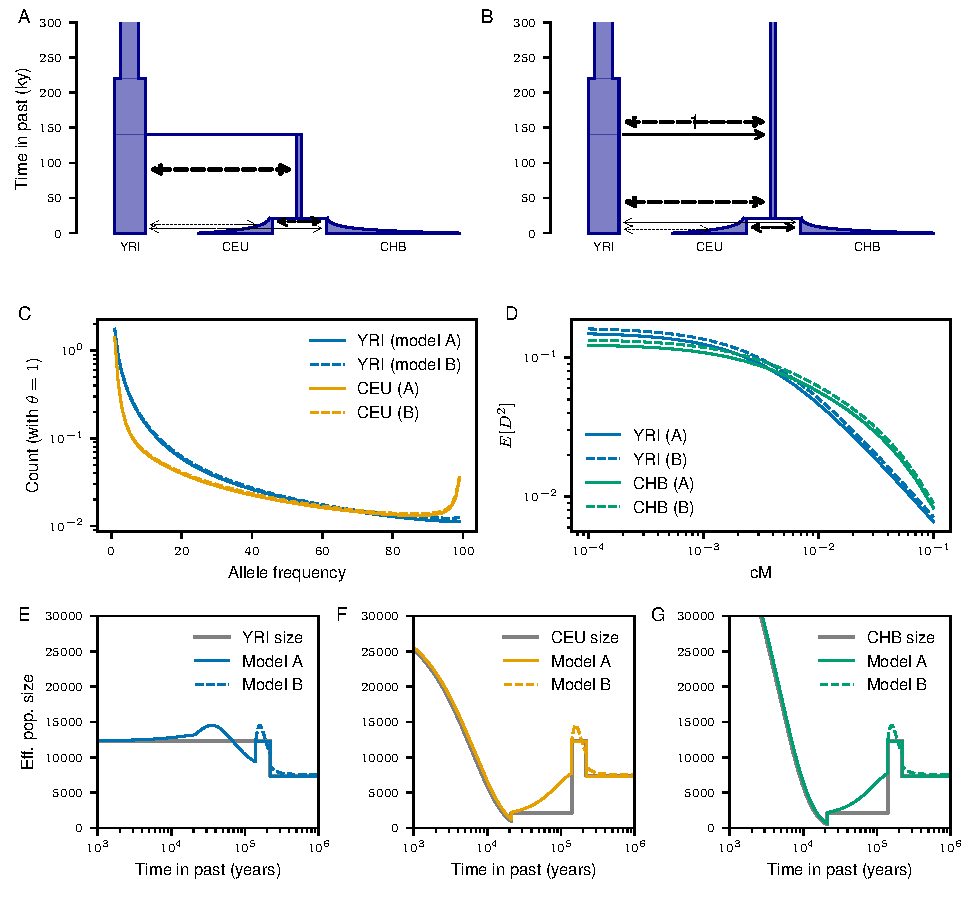
\includegraphics{figures/ooa_expected_stats.pdf}}
\caption{\textbf{Expected diversity statistics under the \citet{gutenkunst2009inferring} model}.
    \textbf{(A)} The correctly implemented model. Dashed arrows depict continuous migration.
    \textbf{(B)} The incorrectly implemented model from the \msprime\ tutorial, with migration continuing
    into the past beyond the mass migration event with proportion $1$ from the ancestral population
    to the bottleneck population.
    \textbf{(C)} Marginal allele frequency spectra under the two models. Heterozygosity in the incorrect model
    is inflated by $~3.5\%$, though the general shape of the distributions are qualitatively similar.
    \textbf{(D)} Similarly, the increased heterozygosity leads to excess $D^2$, though the LD-decay is
    qualitatively similar between models.
    \textbf{(E-G)} True size history for each population plotted against the expected size history from
    the expected inverse coalescence rates.
}
\label{fig:ooa_stats}
\end{center}
\end{figure}

\begin{figure}[ht]
\begin{center}
\makebox[\textwidth][c]{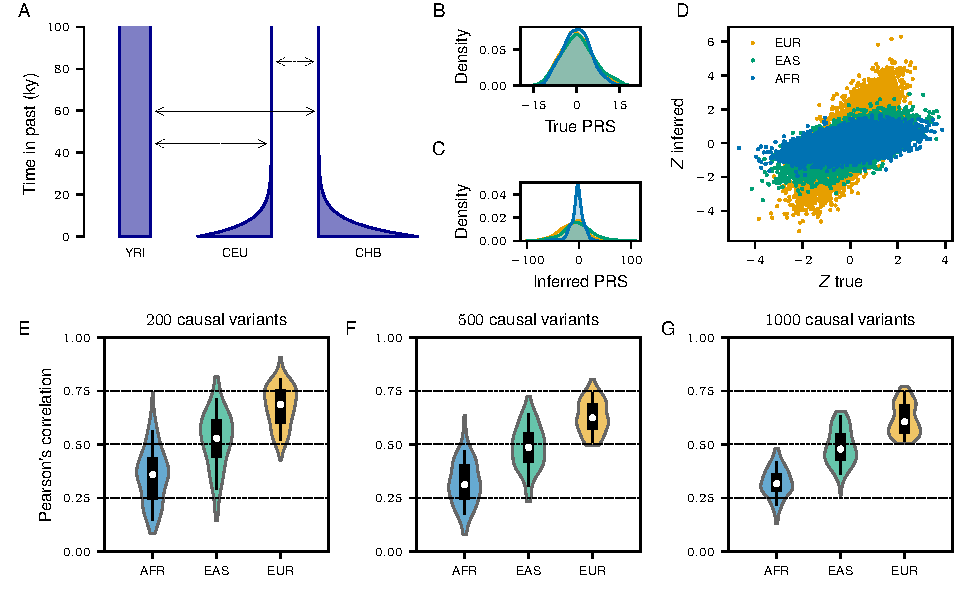
\includegraphics{figures/prs_fig.pdf}}
\caption{\textbf{The transferability of PRS under neutrality}.
    \textbf{(A)} In~\citet{martin2017human}, the simulated demographic model did not apply demographic
    events in the past, so continental populations were simulated as isolated with low levels of migration
    for all time. The intended model is shown in Figure \ref{fig:ooa_stats}A.
    \textbf{(B-G)} We repeated the simulation experiment in~\cite{martin2017human} using the correct
    demographic model.
    While risk prediction in the African and East Asian population is reduced compared to the studied
    European population, the reduction in prediction accuracy is not as hopeless as originally reported.
    Notably, under a neutral polygenic architecture, we do not expect significant bias in inferred PRS
    in any of the populations (C, D).
    Correlations were computed over 100 simulation replicates.
    For direct comparison to the original study, see Figure~5 in~\citet{martin2017human}.
}
\label{fig:prs}
\end{center}
\end{figure}

\end{document}
